\chapter{数据基础与问题分析}

\section{数据来源与总体说明}

本文研究数据来源于与美国哈里伯顿公司开展的横向合作项目。本研究基于哈里伯顿公司提供的同一井段 XSI 阵列声波测井数据、CAST 超声成像测井数据和工具姿态相关数据，分析声波响应与套管外水泥环状态之间的关系。为避免披露与研究目标无关的信息，本文只给出数据结构、井段范围和必要的处理参数，不公开井名、地理位置及生产信息。

研究井段为 2732--4132~ft。主要数据包括：XSI 多接收器全波列、CAST 声阻抗矩阵，以及与 XSI 深度对应的 Relative Bearing 和 Inclination。XSI、CAST 和姿态数据分别具有不同的采样间隔和记录顺序，本研究先核验各自深度轴，再在 0.1~ft 派生深度网格上构造样本。该网格是本研究的数据处理参数，不是仪器原始采样分辨率。

数据核验采用项目 MAT 文件、处理代码、配置文件、汇报材料和公开工具论文相互印证。公开工具论文用于说明接收器几何和一般测量原理，项目文件用于确定本研究实际使用的数组维度和处理参数。二者发生差异时，以“仪器结构”和“本文数据子集”分别表述，避免把处理窗口写成仪器能力。

\begin{table}[htbp]
  \centering
  \small
  \setlength{\tabcolsep}{4pt}
  \caption{本文使用的主要数据及其原始组织}
  \label{tab:data-overview}
  \begin{tabular}{p{0.20\textwidth}p{0.25\textwidth}p{0.22\textwidth}p{0.23\textwidth}}
    \toprule
    数据 & 主要变量 & 原始数组 & 本文用途 \\
    \midrule
    XSI 第 3 接收环 & Depth、Tad、SideA--SideH & 每个侧向波形矩阵为 $1024\times7108$ & 构造 8 通道 CWT 输入 \\
    CAST & Depth、$Z_c$ & $Z_c$ 为 $180\times24750$ & 构造深度--方位参考标签 \\
    工具姿态 & Depth、Inc、RelBearing & 三个长度均为 13508 的向量 & 分析井斜与相对方位可靠性 \\
    \bottomrule
  \end{tabular}
\end{table}

在目标井段内，XSI 第 3 接收环共有 2852 条深度记录，其中 2846 个深度值唯一；CAST 对应 9884 个深度记录；姿态数据对应 5549 条记录。数据量差异来自工具采样方式，不代表一一对应关系。最终回归实验按共同有效范围和样本窗口形成 2842 个候选样本，其中 19 个位于划分缓冲区，不参与训练、验证或测试。

\section{XSI 声波测井数据结构}

\subsection{工具几何与数据子集}

XSI 类超宽带阵列声波工具通过多个单极和偶极声源激发井内波场，并由轴向、周向分布的接收器记录波形。公开工具论文给出的接收段包含 13 个轴向接收环，每环 8 个接收器沿周向等间隔布置，共 104 个接收器\cite{Sun2016UltrabroadbandAcoustic}。13 个接收环提供不同源距，8 个周向单元提供工具坐标系内的方位采样。这里的“$13\times8$”描述仪器接收器几何，不等于本文模型输入维度。

项目数据按接收环拆分。本文使用第 3 接收环，对应 SideA 至 SideH 共 8 个周向通道；其余接收环不进入本轮模型。项目配置给出的 13 个接收环相对源偏移从 3~ft 到 $-3$~ft，以 0.5~ft 递减，第 3 接收环偏移为 2~ft。接收器字母只表示工具内部的周向编号。除非同时知道工具姿态和每个字母相对参考方向的定义，SideA 不能直接解释为北向、井眼高边或 CAST 图像零点\cite{Che2014PhasedArcReception,Che2017AzimuthalReceiver}。

\subsection{时间采样与分析窗口}

第 3 接收环每个侧向通道的原始波形长度为 1024 点，存储类型为 32 位整数。项目数据采样率为 100~kHz，对应采样间隔为 10~$\mu$s，单条原始波形记录时长约为 10.24~ms。本文仅选取每条波形的前 400 点，即约 4~ms，用于覆盖研究所关注的早期声波响应。400 点是本文的预处理窗口，不能表述为仪器只能采集 400 点。

100~kHz 采样率对应 50~kHz 的奈奎斯特频率，但奈奎斯特频率不等于仪器换能器的有效响应范围。本文 CWT 采用 1--30~kHz 的分析频带，该范围由项目处理配置确定。公开工具论文展示了不同发射模式和处理频带\cite{Sun2016UltrabroadbandAcoustic}，但本文不据此推定本项目仪器的原始带宽；1--30~kHz 仅表示本文选取的 CWT 分析频带。

\subsection{深度轴、异常值与张量维度}

XSI 第 3 接收环在目标井段的唯一深度间隔中位数约为 0.493~ft，存在 9 个重复深度以及少量局部顺序变化。处理时先按深度排序、合并重复索引，再映射到统一网格。8 个通道的原始矩阵均为有限整数，未发现 NaN 或 Inf。原始 XSI 波形中存在少量达到有符号 24 位数字量程上下限的采样点，其数值分别为 $-8388608=-2^{23}$ 和 $8388607=2^{23}-1$，表现为局部采集饱和或数字削顶。模型实际输入范围内共检测到 156 个端点采样值，其中下限值 109 个、上限值 47 个，涉及 75 条深度记录。没有证据表明这些端点是缺测编码。

历史预处理没有对上述端点值执行专门的掩膜、替换或人工裁剪，而是将前 400 点直接送入 1~kHz 四阶零相位高通。滤波结果保持有限，但线性滤波不等同于对削顶波形的恢复。由于端点数量在整体输入数据中极少，经项目数据核查，其对模型总体实验结果的影响可以忽略；本文仍将其作为原始采集数据的质量现象予以说明，不将“影响可以忽略”表述为“完全没有影响”。

单个深度样本经 1~kHz 四阶零相位高通、前 400 点截取和复 Morlet CWT 后，每个通道形成 $150\times400$ 的时间--频率图。8 个周向通道堆叠后，模型输入张量为
\begin{equation}
  \mathbf{X}\in\mathbb{R}^{150\times400\times8},
  \label{eq:xsi-input-shape}
\end{equation}
其中 150 为尺度或频率采样数，400 为时间采样数，8 为第 3 接收环的周向通道数。

\begin{table}[htbp]
  \centering
  \caption{XSI 原始参数与本文处理参数的区分}
  \label{tab:xsi-parameters}
  \begin{tabular}{p{0.32\textwidth}p{0.25\textwidth}p{0.32\textwidth}}
    \toprule
    项目 & 核验值 & 属性 \\
    \midrule
    接收器几何 & 13 环，每环 8 个接收器 & 公开工具结构 \\
    本文接收环 & 第 3 环，SideA--SideH & 研究数据子集 \\
    原始波形长度 & 1024 点 & 项目 MAT 文件 \\
    时间采样间隔 & 10~$\mu$s & 项目数据采样参数 \\
    本文时间窗 & 前 400 点，4.00~ms & 预处理参数 \\
    采样率/奈奎斯特频率 & 100/50~kHz & 项目配置/数学上限 \\
    本文 CWT 频带 & 1--30~kHz & 特征提取参数 \\
    CWT 输入维度 & $150\times400\times8$ & 模型输入 \\
    \bottomrule
  \end{tabular}
\end{table}

\section{CAST 超声成像数据结构}

\subsection{测量原理与矩阵组织}

CAST 数据以超声脉冲回波测量为基础。换能器向套管内壁发射脉冲，回波的到达、幅度和共振衰减受套管厚度、井液以及套管后介质影响。通过周向扫描，可将套管后介质的等效声阻抗按深度和方位排列为图像。脉冲回波、弯曲波和传统声波胶结测量对不同波模态敏感，解释时应结合其适用条件\cite{Froelich1982CementEvaluation,Froelich2008MultimodeCement,Wang2016AcousticCementMethods}。

声阻抗通常定义为
\begin{equation}
  Z=\rho c,
  \label{eq:acoustic-impedance}
\end{equation}
其中 $\rho$ 为介质密度，$c$ 为声速。套管与套管后介质的阻抗和界面耦合共同影响回波。低声阻抗响应可能与液体通道或胶结较差有关，但不能仅凭一个像素断言其对应真实窜槽。

CAST 数据中的 $Z_c$ 表示套管外介质的声阻抗，单位为 MRayl。项目 \texttt{CAST.mat} 中的 $Z_c$ 矩阵为 $180\times24750$，第一维为周向采样，第二维为深度。每个深度位置包含 180 个等角度方位采样点，相邻方位间隔为 $2^\circ$，完整覆盖井周 $360^\circ$。深度从约 2395.445~ft 延伸到 5804.337~ft，在目标井段内有 9884 个记录，深度间隔中位数约为 0.142~ft。完整周向覆盖和采样间隔已经确认，但现有数据不包含可将 CAST 方位零点唯一转换到 XSI 通道零点的共同参考信息。

\subsection{数值质量与派生标签}

$Z_c$ 矩阵中的 4,455,000 个元素均为有限数值，没有 NaN 或 Inf；全数据中有 14 个负值。根据项目事实，负声阻抗缺乏合理物理意义，应视为无效值。历史预处理代码并未对它们显式掩膜、替换、裁剪或插值修复，而是先按深度对整幅 $Z_c$ 线性插值。数据复核表明，这 14 个原始负值分布于 2469.003--2504.845~ft 和 4898.053~ft，全部位于本文 2732--4132~ft 目标井段之外；目标井段原始数据和 0.1~ft 插值网格中均没有负值。因此，这些无效值没有进入本文的一维占比标签或 FFT 幅值标签，也没有影响已完成实验指标。该结论来自位置与代码链核查，不能改写成“历史代码已经执行负值掩膜”。

根据美国哈里伯顿公司在本项目 CAST 成像解释中采用的数据判别约定，本文选取 $Z_c=2.5~\mathrm{MRayl}$ 作为参考阈值。该数值并非本文自行提出或通过优化得到，也不是适用于所有工具、井况和水泥体系的普适行业标准。由该阈值得到的严重度和结构标签属于参考工具成像结果的派生表征，既不是直接测量得到的绝对真实标签，也不能解释为绝对窜槽宽度或缺陷体积。

\section{XSI--CAST 方位失配问题分析}

\subsection{需要区分的坐标量}

方位关系分析中需要区分六类量：

\begin{enumerate}
  \item 仪器方位：工具坐标系相对某一外部参考方向的转角；
  \item 接收器编号：SideA--SideH 在工具圆周上的相对位置；
  \item 井眼高边：倾斜井眼横截面中重力意义上的上方方向；
  \item Relative Bearing：工具某参考轴相对于指定参考方向的周向角；
  \item Inclination：井眼或工具轴相对铅垂方向的倾角；
  \item CAST 与 XSI 方位零点：两套数据周向索引各自的起始方向。
\end{enumerate}

方位阵列文献通常在接收器几何和参考方向已知时讨论入射方向或窜槽方位\cite{Che2014PhasedArcReception,Che2017AzimuthalReceiver,Zuo2020AzimuthCement}。本文虽然知道八个 XSI 通道以 $45^\circ$ 相对间隔布置，但缺少 CAST 零点和 XSI 工具参考轴之间的唯一对应。相对间隔已知不等于绝对起点已知。

\subsection{Inclination 数据分析}

目标井段 Inclination 的最小值为 $0.1349^\circ$，最大值为 $2.2879^\circ$，均值为 $0.5218^\circ$，中位数为 $0.4705^\circ$；5\%--95\% 分位范围约为 $0.2097^\circ$--$1.1975^\circ$。这说明研究井段总体接近直井。在接近铅垂时，井眼高边方向对微小姿态和测量噪声更敏感。

Inclination 是工具轴相对铅垂方向的倾角大小，不包含绕工具轴旋转的方向信息。即使倾角测量完全可靠，也不能由一个标量倾角推导 XSI 方位零点相对 CAST 零点的旋转。因此，Inclination 不能直接作为方位校正角。

\begin{figure}[htbp]
  \centering
  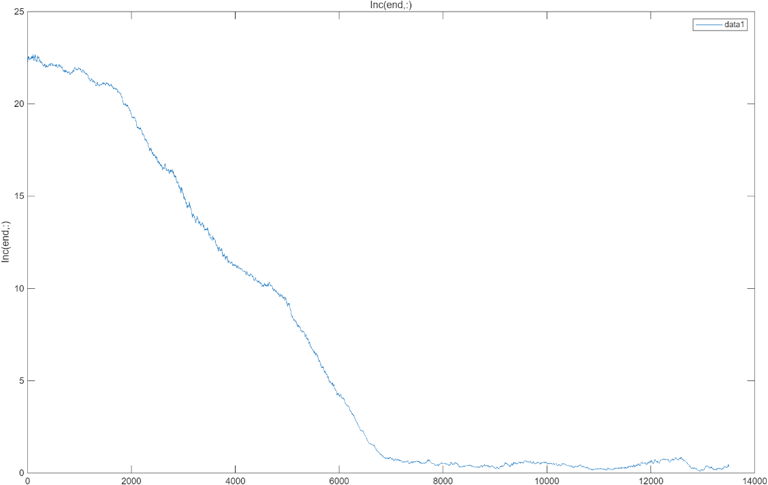
\includegraphics[width=0.78\textwidth]{figures/revision/inclination.png}
  \caption{Inclination 随记录索引的变化。目标井段总体接近直井}
  \label{fig:inclination}
\end{figure}

\subsection{Relative Bearing 数据分析}

在 2732--4132~ft 目标井段内，Relative Bearing 范围约为 $1.85^\circ$--$357.82^\circ$。按圆周差计算，相邻记录绝对变化的中位数为 $5.156^\circ$，95\% 分位为 $28.639^\circ$，99\% 分位为 $64.611^\circ$，最大值为 $178.563^\circ$；其中 111 次变化超过 $45^\circ$，23 次超过 $90^\circ$。图 \ref{fig:relative-bearing} 显示，接近直井的区间存在明显跳变，而井斜增大后的区间更平滑。该现象与项目汇报中“近直井段 Relative Bearing 可靠性较低”的记录一致。

\begin{figure}[htbp]
  \centering
  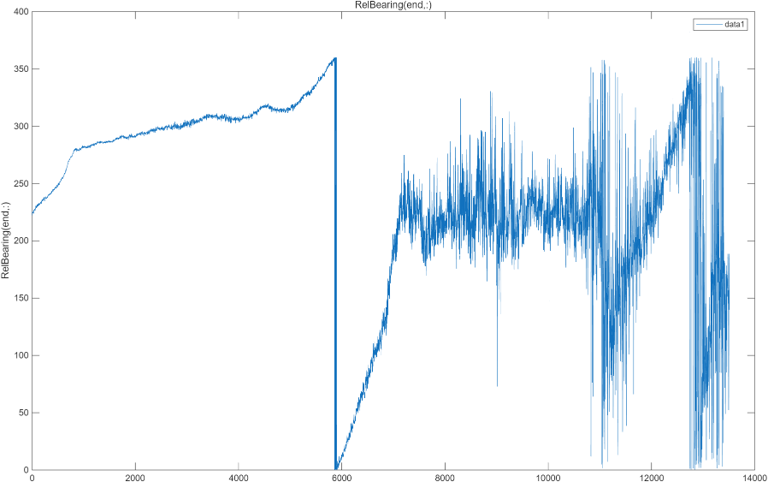
\includegraphics[width=0.78\textwidth]{figures/revision/relative_bearing.png}
  \caption{Relative Bearing 随记录索引的变化。接近直井区间存在较多周向跳变}
  \label{fig:relative-bearing}
\end{figure}

然而，当前 MAT 文件没有给出 Relative Bearing 的正式参考方向定义，也没有给出 CAST 方位零点。仅凭曲线连续性无法判断某一数值对应磁北、井眼高边、工具面还是其他处理约定。受现有工具姿态元数据和方位基准信息限制，本文无法建立两类测井数据绝对方位零点之间的唯一转换关系。

\subsection{深度差异与标签误差}

XSI、CAST 和姿态数据的原始深度采样分别约为 0.493、0.142 和 0.25~ft 的量级，并存在局部重复、重排或间隔变化。深度插值可以把三类数据映射到共同网格，却不能补充缺失的方位零点。若在没有绝对零点转换的条件下，把 CAST 第 $j$ 个方位像素直接赋给 XSI 第 $j$ 个通道，同一物理结构可能因未知循环移位而对应不同标签。这种误差不是增加样本量即可自动消除的随机噪声，而是与工具姿态相关的系统性标签不一致。

本文大部分实验使用 2732--4132~ft 井段。该井段 Inclination 中位数仅为 $0.4705^\circ$，整体接近直井；与此同时，Relative Bearing 呈现频繁且幅度较大的跳变，Inclination 又只描述井斜大小，不能充当绕工具轴的旋转校正角。结合 XSI 与 CAST 绝对方位零点之间缺少唯一转换关系这一事实，本文不把 CAST 的绝对方位位置作为监督目标，也不建立未经证据支持的绝对角度公式。

对 CAST 的 180 点完整周向序列，未知方位零点差异在离散表示上建模为循环平移。第三章沿方位维进行离散傅里叶变换并使用幅值：循环移位改变相位而不改变幅值，从而降低未知方位移位的影响。该标签保留环向结构的频率组成，但舍弃绝对方位位置和相位信息；它不能恢复窜槽的绝对方位，也不能替代可靠的工具姿态配准。

\section{相邻深度相关性与验证边界}

声波和 CAST 标签均由连续深度窗口构造，相邻样本可能共享相近地层、套管条件和重叠窗口。对这类结构化数据进行随机划分，训练集与测试集容易包含邻近深度，从而低估预测误差\cite{Roberts2017CrossValidation,Valavi2019BlockCV}。本文将随机样本划分用于先导可学习性检验，将主要回归结论建立在单井深度区间隔离划分上。

严格划分中，训练集为 1984 个样本，深度范围 2732.440--3715.853~ft；验证集为 416 个样本，范围 3721.119--3917.685~ft；测试集为 423 个样本，范围 3922.785--4129.744~ft。相邻集合之间设置 5~ft 缓冲区，共排除 19 个样本。三个集合的深度键无交集。该设置提高了同井验证的严格程度，但仍不能代替跨井验证。

\section{本章小结}

本章从项目文件、已确认项目事实和公开工具论文核验了 XSI、CAST 与姿态数据。XSI 工具具有 13 环、每环 8 个接收器的结构，共 104 个接收通道，而本文仅使用第 3 接收环的 8 通道、前 400 点波形；少量 24 位端点削顶对总体实验结果的影响可以忽略，但仍作为数据质量现象保留说明。CAST 声阻抗单位为 MRayl，由 180 个按 $2^\circ$ 等间隔覆盖完整井周的方位点和不规则深度轴组成，其 $2.5~\mathrm{MRayl}$ 阈值是哈里伯顿公司在本项目成像解释中采用的项目约定。Inclination 只表示井斜大小，Relative Bearing 在目标近直井段存在频繁跳变，且两类工具缺少可相互转换的绝对方位零点。上述事实构成不使用绝对方位位置监督、采用方位向 FFT 幅值标签和深度区间隔离验证的直接依据。
